Pour ce projet, notre robot doit être capable de répondre à trois ordres différents : avance tout droit, tourne à droite, tourne à gauche. Le signal audio que nous lui envoyons doit donc contenir cet ordre ainsi qu'une quantité associée : le nombre de centimètres à parcourir ou le nombre de degré qu'il doit tourner. Dans ce chapitre, nous allons développer le chemin que parcourt l'information entre le moment où elle est envoyée sous forme sonore par l'émetteur qui nous a été fourni et la réception par le microcontrôleur.

\section{Codage de l'ordre}
Le message envoyé au robot est codé sur 13 bits. Le premier et le dernier sont tout deux mis dans l'état bas \SI{0}, ils font office de start bit et de stop bit, c'est-à-dire qu'ils délimitent la commande. L'avant dernier bit est un bit de parité, il permet de détecter les cas où la commande est erronée parce qu'elle contient un nombre impair de bits. Les \SI{10} bits restant contiennent l'information utile, les deux premiers donnent l'ordre suivant la convention suivante :
\begin{itemize}
\item \ilcode{0b00} : avance tout droit
\item \ilcode{0b01} : tourne à droite
\item \ilcode{0b10} : tourne à gauche
\end{itemize}
Les 8 bits suivants représentent simplement le nombre de degrés ou de centimètres à parcourir. Par exemple, la trame \ilcode{0101111111110} fera tourner notre robot de \SI{255}{\degree} dans le sens anti-horlogique.

Pour ce qui est de mettre en forme le signal audio, une fonction Matlab se charge de générer le signal audio modulé en FSK correspondant à l'information que l'on désire envoyer. Le principe de la modulation FSK est simple : la fréquence du signal correspond soit à l'état haut soit à l'état bas. Dans notre cas, chaque bit de la trame d'information sera émis sur une période de \SI{1}{\milli\second}, un bit 1 sera représenté par une fréquence de \SI{1100}{\hertz} et un bit 0 par une fréquence de \SI{900}{\hertz}. 

\section{Notre chaîne d'acquisition}
Notre chaîne d'acquisition est constituée de plusieurs étages :
\begin{itemize}
\item Le micro
\item L'amplification
\item Le filtre de garde
\item Le convertisseur analogique-numérique
\item Les filtres passe-bande
\end{itemize}

\subsection{Le micro}
Notre microphone fournit un signal d'une amplitude maximale de \SI{1}{\milli\volt}. Pour le faire fonctionner il a fallu le polariser avec une résistance de \SI{2.2}{\kilo\ohm} suivant le schéma de la figure \ref{fig:polarisation du micro}.

\begin{figure}[htbp]
\centering
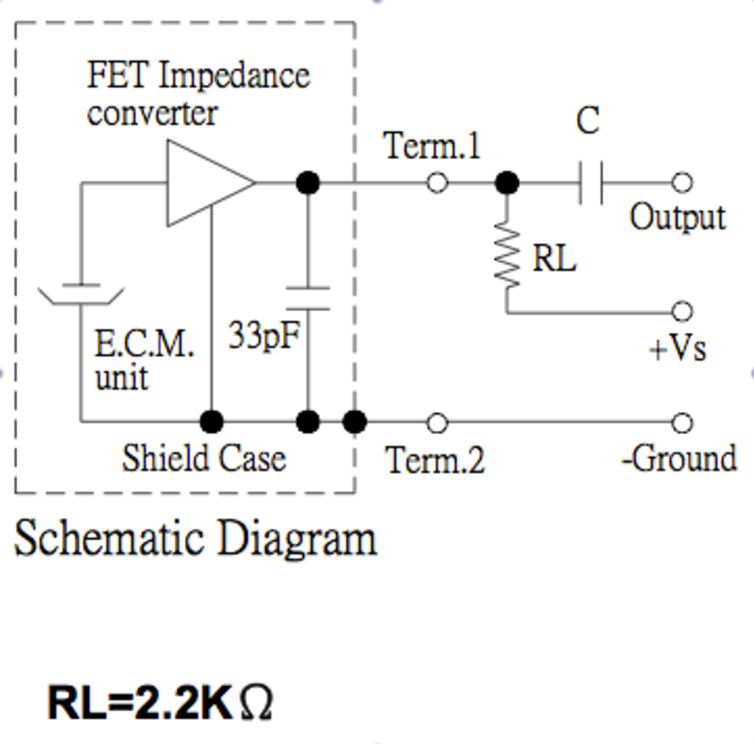
\includegraphics[width=0.7\textwidth]{polarisation_micro.pdf}
\caption{Circuit du microphone}
\label{fig:polarisation du micro}
\end{figure}
Le principe de fonctionnement du micro est que sa membrane extérieure mobile constitue l'armature d'un condensateur chargé en permanence, la deuxième armature étant fixe. Le mouvement de cette membrane, dû aux variations de pression, va modifier la capacité du condensateur, et donc la tension à ses bornes. Le microphone est dit piézoélectrique. Dans notre cas, le microphone est aussi dit "à électret", ce qui signifie qu'il ne nécessite pas d'alimentation pour maintenir le condensateur chargé : le matériau constituant la membrane présente la propriété de conserver une charge électrostatique. Cependant, une alimentation est nécessaire pour polariser le transistor de l'étage de sortie du microphone, au travers de la résistance $R_L$. 

\subsection{Montage amplificateur}
Comme nous l'avons dit précédemment, le signal en sortie de notre micro a une amplitude maximale de \SI{1}{\milli\volt}. La plage des tensions d'entrée de l'ADC va de \SI{0}{\volt} à \SI{3.3}{\volt}, afin d'occuper cette plage le plus largement possible tout en gardant une marge de sécurité par rapport à la saturation de l'ADC, il nous était demandé de traiter notre signal de façon à le centrer sur \SI{1.65}{\volt} et atteindre une valeur crête à crête de \SI{3}{\volt}. Pour cela nous avons utilisé deux étages amplificateurs, respectivement d'un gain de 68 et 22. Nous avons donc utilisé le montage représenté à la figure \ref{fig:etage amplificateur}. 

Calculons d'abord la tension à la sortie du premier étage ($V_{out 1}$), à l'aide du principe de superposition. On considère d'abord la seule source de tension continue, la capacité est alors un circuit ouvert (\ref{eqn:2.1}):
\begin{figure}
\centering
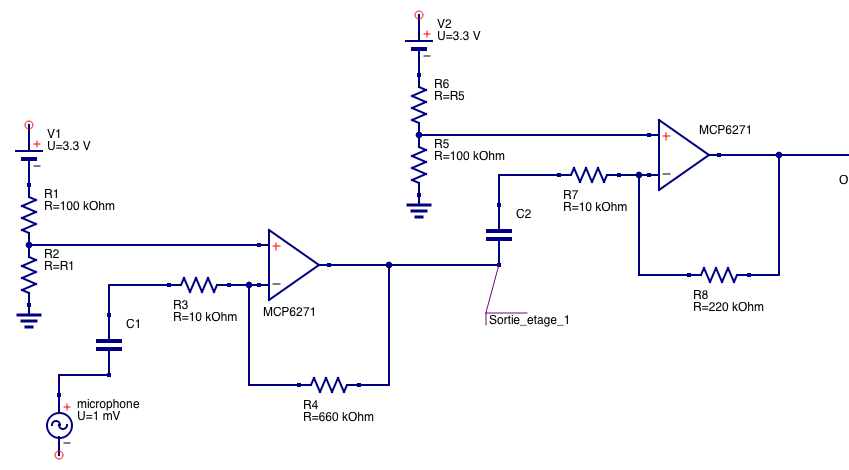
\includegraphics[width=0.7\textwidth]{etage_amplificateur.png}
\caption{Etage amplificateur}
\label{fig:etage amplificateur}
\end{figure}
\begin{equation}
V_{+} = V_{-} = V_{out 1} = \SI{1.65}{\volt}
\label{eqn:2.1}
\end{equation}
Considérons ensuite uniquement la source de tension continue, le circuit est alors un inverseur classique (\ref{eqn:2.2}) : 
\begin{equation}
V_{out 1} = \frac{R_2}{R_1} V_{micro} = 68 V_{in}
\label{eqn:2.2}
\end{equation}
On retrouve la tension en sortie du premier étage en sommant ces deux termes pour finalement obtenir (\ref{eqn:2.3}) :
\begin{equation}
V_{out 1} = \SI{1.65}{\volt} + 68 V_{micro}
\label{eqn:2.3}
\end{equation}

La capacité $C_{2}$ placée entre nos deux étages d'amplification sert à supprimer la composante continue de la tension, la recentrant autour de \SI{0}{\volt}. On évite ainsi de faire saturer notre deuxième ampli-op. Pour le deuxième étage, les calculs sont exactement les mêmes que pour le premier, exception faite du gain du montage inverseur qui vaut 22. On obtient alors notre signal amplifié (\ref{eqn:2.4}) : 
\begin{equation}
V_{out final} = \SI{1.65}{\volt} + 1496 V_{micro}
\label{eqn:2.4}
\end{equation}

Pour être persuadé du bon fonctionnement de notre étage amplificateur, nous avons bien sûr effectué des essais sur celui-ci au départ du générateur de fréquences mis à notre disposition. Les résultats obtenus à l'oscilloscope sont entièrement satisfaisants. 

\subsection{Filtre de garde}
